% !TeX root = ../main.tex

\subsection*{3.2 Frequency response}

In the graph below we observe the Bode plot of the transfer functions
$G(s)=\dfrac{1}{(s+1)(0.5s+1)}$ and $G_c(s)=\dfrac{-s+c}{c\,(s+1)(0.5s+1)}$ for $c=-10,\,-0.25,\,-0.1,\,0.1,\,0.25,\,10$.
The zero of $G_c$ sits at $s=c$, and dividing by $c$ keeps the DC gain at 1, so only the zero placement changes between systems.

\begin{figure}[H]
\centering
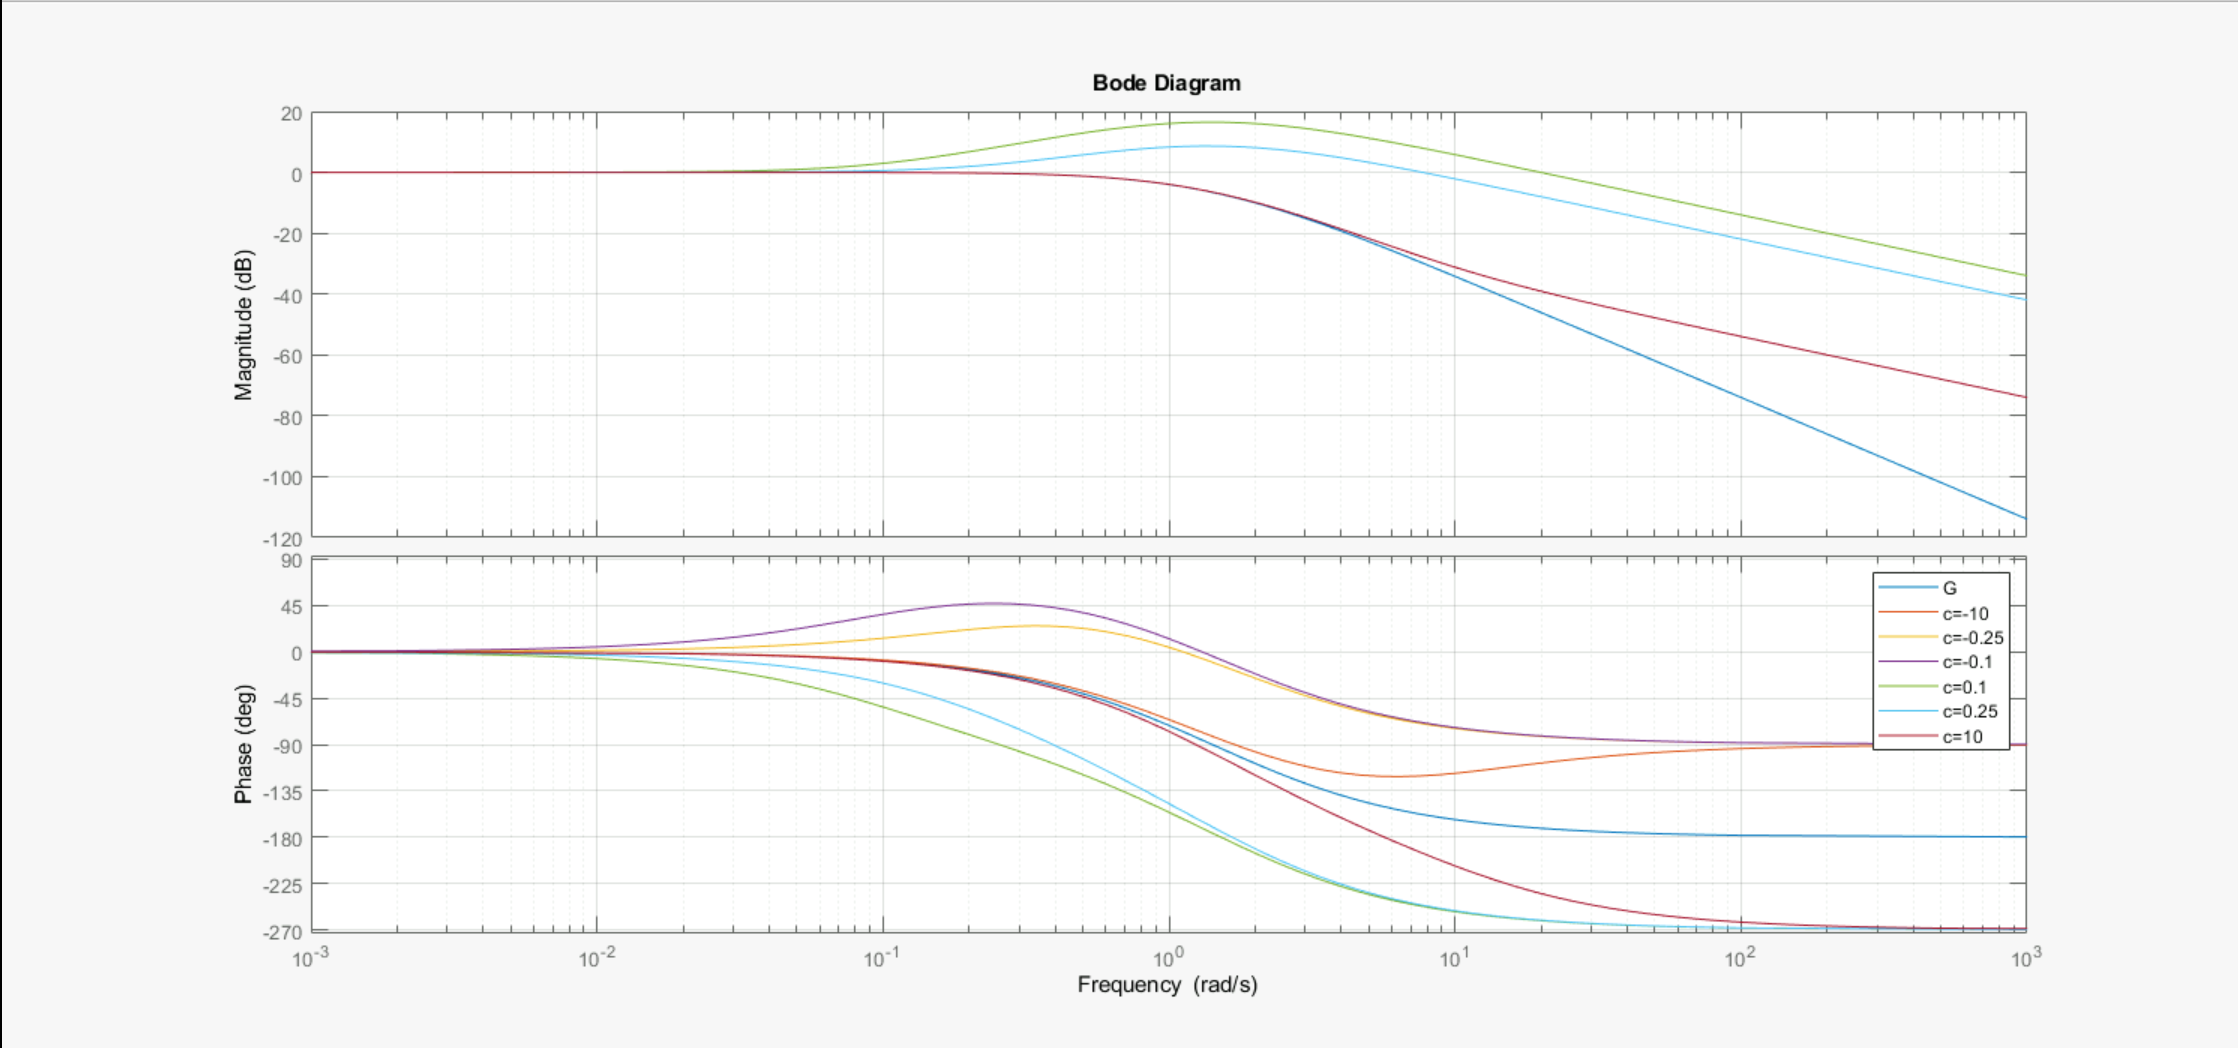
\includegraphics[width=0.58\textwidth]{figures/3_2/bode_plot_all.png}
\caption{Bode plot of $G(s)$ and the six $G_c(s)$, phase offset adjusted.}
\end{figure}

In the figure we observe that the magnitude of $G_c(s)$ with the same $|c|$ is the same curve 
(explained below), while each phase curve is distinct. The phases all begin at $0^\circ$ because 
the ``Adjust Phase Offset'' feature was used to make a fair comparison. Zeros with $c<0$ 
(left half-plane) give a phase lead, so their curves sit above $G(s)$, and zeros with $c>0$ (right half-plane) 
give a phase lag, so their curves sit below $G(s)$. This follows from the maths: $G_c(s)=\left(1-\tfrac{s}{c}\right)G(s)$, 
so at $s=j\omega$ the zero adds $\angle\!\left(1-\tfrac{j\omega}{c}\right)=-\arctan(\omega/c)$ to the phase of $G$. 
For $c=-\alpha$ this is $+\arctan(\omega/\alpha)$ (lead) and for $c=+\alpha$ it is $-\arctan(\omega/\alpha)$ (lag).
 
\begin{table}[H]
\centering\small
\begin{tabular}{@{}clrrr@{}}
\toprule
Group ($\alpha$) & Transfer function & $\omega=0$ & $\omega=\alpha$ & $\omega\gg\alpha$ \\ \midrule
1 (0.1)  & $G(s)$        & 0.00 & $-8.65$   & $-180.00$ \\
         & $G_{c=0.1}(s)$  & 0.00 & $-53.60$  & $-270.00$ \\
         & $G_{c=-0.1}(s)$ & 0.00 & $36.30$   & $-90.00$ \\ \addlinespace
2 (0.25) & $G(s)$        & 0.00 & $-21.10$  & $-180.00$ \\
         & $G_{c=0.25}(s)$ & 0.00 & $-66.20$  & $-270.00$ \\
         & $G_{c=-0.25}(s)$& 0.00 & $23.80$   & $-90.00$ \\ \addlinespace
3 (10)   & $G(s)$        & 0.00 & $-163.00$ & $-180.00$ \\
         & $G_{c=10}(s)$   & 0.00 & $-208.00$ & $-270.00$ \\
         & $G_{c=-10}(s)$  & 0.00 & $-118.00$ & $-90.00$ \\ \bottomrule
\end{tabular}
\caption{Phase (degrees) read from the Bode plots (Appendix) for each triple.}
\end{table}
 
In section two we compare the transfer functions with the same $|c|$ against $G(s)$, for example $G_{c=-10}$, $G_{c=10}$ and $G$. 
The results are in the table above. In each figure of the appendix we see two curves in the magnitude plot and three in the phase plot. 
This is because the sign of the zero does not change the magnitude:
$$\left|1+\tfrac{j\omega}{\alpha}\right|=\sqrt{1+\tfrac{\omega^2}{\alpha^2}}=\left|1-\tfrac{j\omega}{\alpha}\right|.$$
Above $\omega=\alpha$ both add $+20$~dB/decade to the gain of $G$.
 
In the table, at $\omega=0$ all three have the same phase of about $0^\circ$. As frequency increases the phase curves separate. 
At $\omega=\alpha$, $G_{c<0}$ has gained a lead of approximately $45^\circ$ on $G$ and $G_{c>0}$ lags $G$ by approximately $45^\circ$, 
so $G_{c>0}$ lags $G_{c<0}$ by $90^\circ$ (e.g.\ $\alpha=10$: $-118^\circ$, $-163^\circ$, $-208^\circ$). For $\omega\gg\alpha$ the gap widens: 
$G_{c<0}$ leads $G$ by $90^\circ$ and $G_{c>0}$ lags it by $90^\circ$, giving a difference of $180^\circ$. 
In general the gap is $2\arctan(\omega/\alpha)$. The size of $\alpha$ matters too. The poles are at 1 and 2 rad/s, so for $\alpha=10$ the zero 
acts well after the poles and the three curves are close in the useful band. For $\alpha=0.25$ and $0.1$ the zero acts first, giving a large gain 
increase and a large phase difference at low frequency.
 
\textbf{Non-minimum phase.} Since $G_{c=\alpha}(s)=G_{c=-\alpha}(s)\cdot\dfrac{\alpha-s}{\alpha+s}$ and the last factor has magnitude 1 at every 
frequency but phase $-2\arctan(\omega/\alpha)$, the right half-plane zero gives the same gain as the left half-plane zero with extra phase lag. 
The system with all poles and zeros in the left half-plane has the least phase lag for a given gain curve, which is the minimum phase system. 
One with the same gain but more lag is therefore called non-minimum phase. This is the same zero that causes the undershoot in 3.1, 
and the extra lag reduces the phase margin, making it harder to control.
 
\newpage
\section*{\large Appendix}
The cursor readings at $\omega=\alpha$ in the table were taken from the plots below. Figure A1 shows the procedure; 
it was done for each triple. The $\omega\gg\alpha$ column is the high-frequency limit of each curve.
 
\begin{figure}[H]
\centering
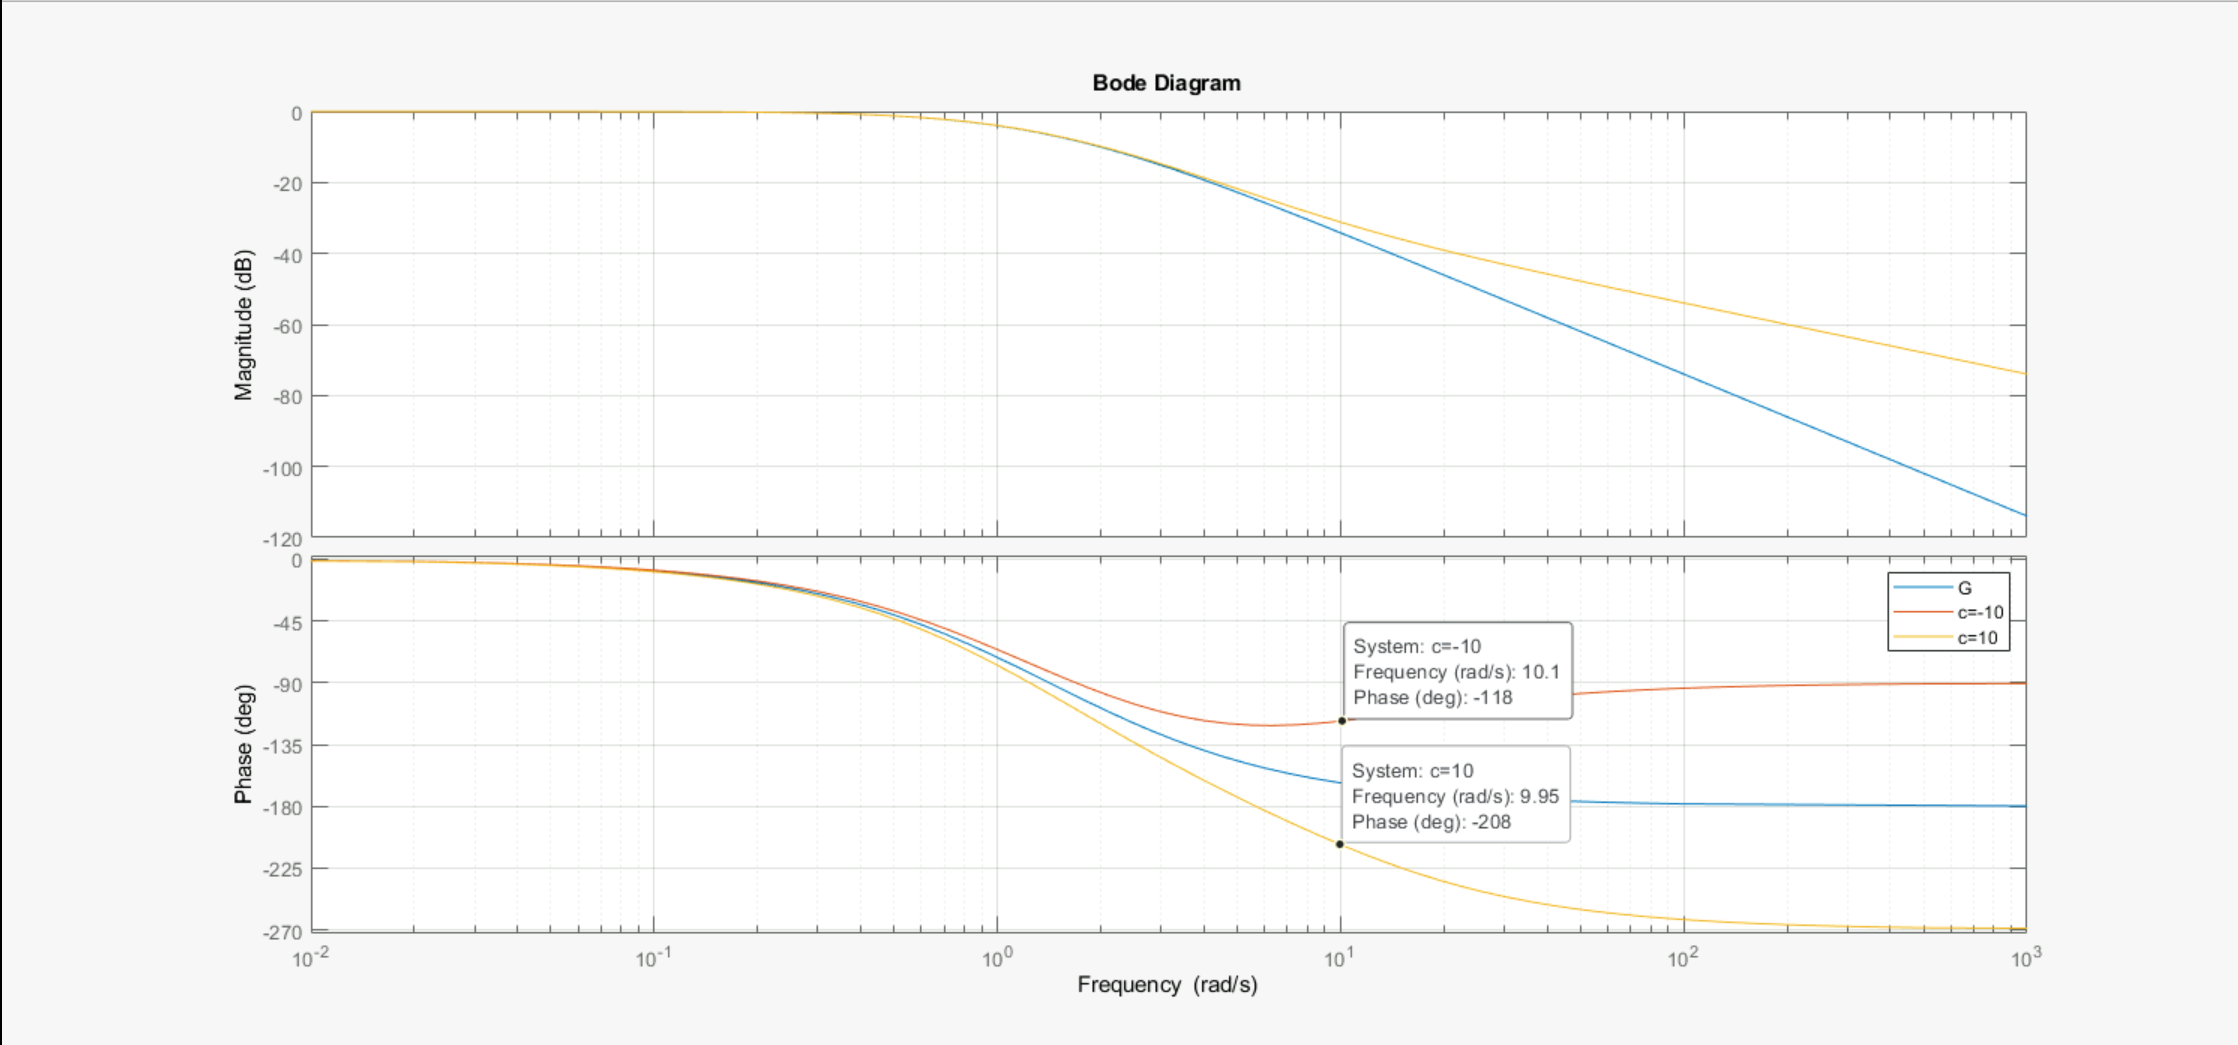
\includegraphics[width=0.75\textwidth]{figures/3_2/test_procedure.png}
\caption*{A1: $G$, $G_{c=-10}$, $G_{c=10}$ ($\alpha=10$), with readings at $\omega=\alpha$.}
\end{figure}
\begin{figure}[H]
\centering
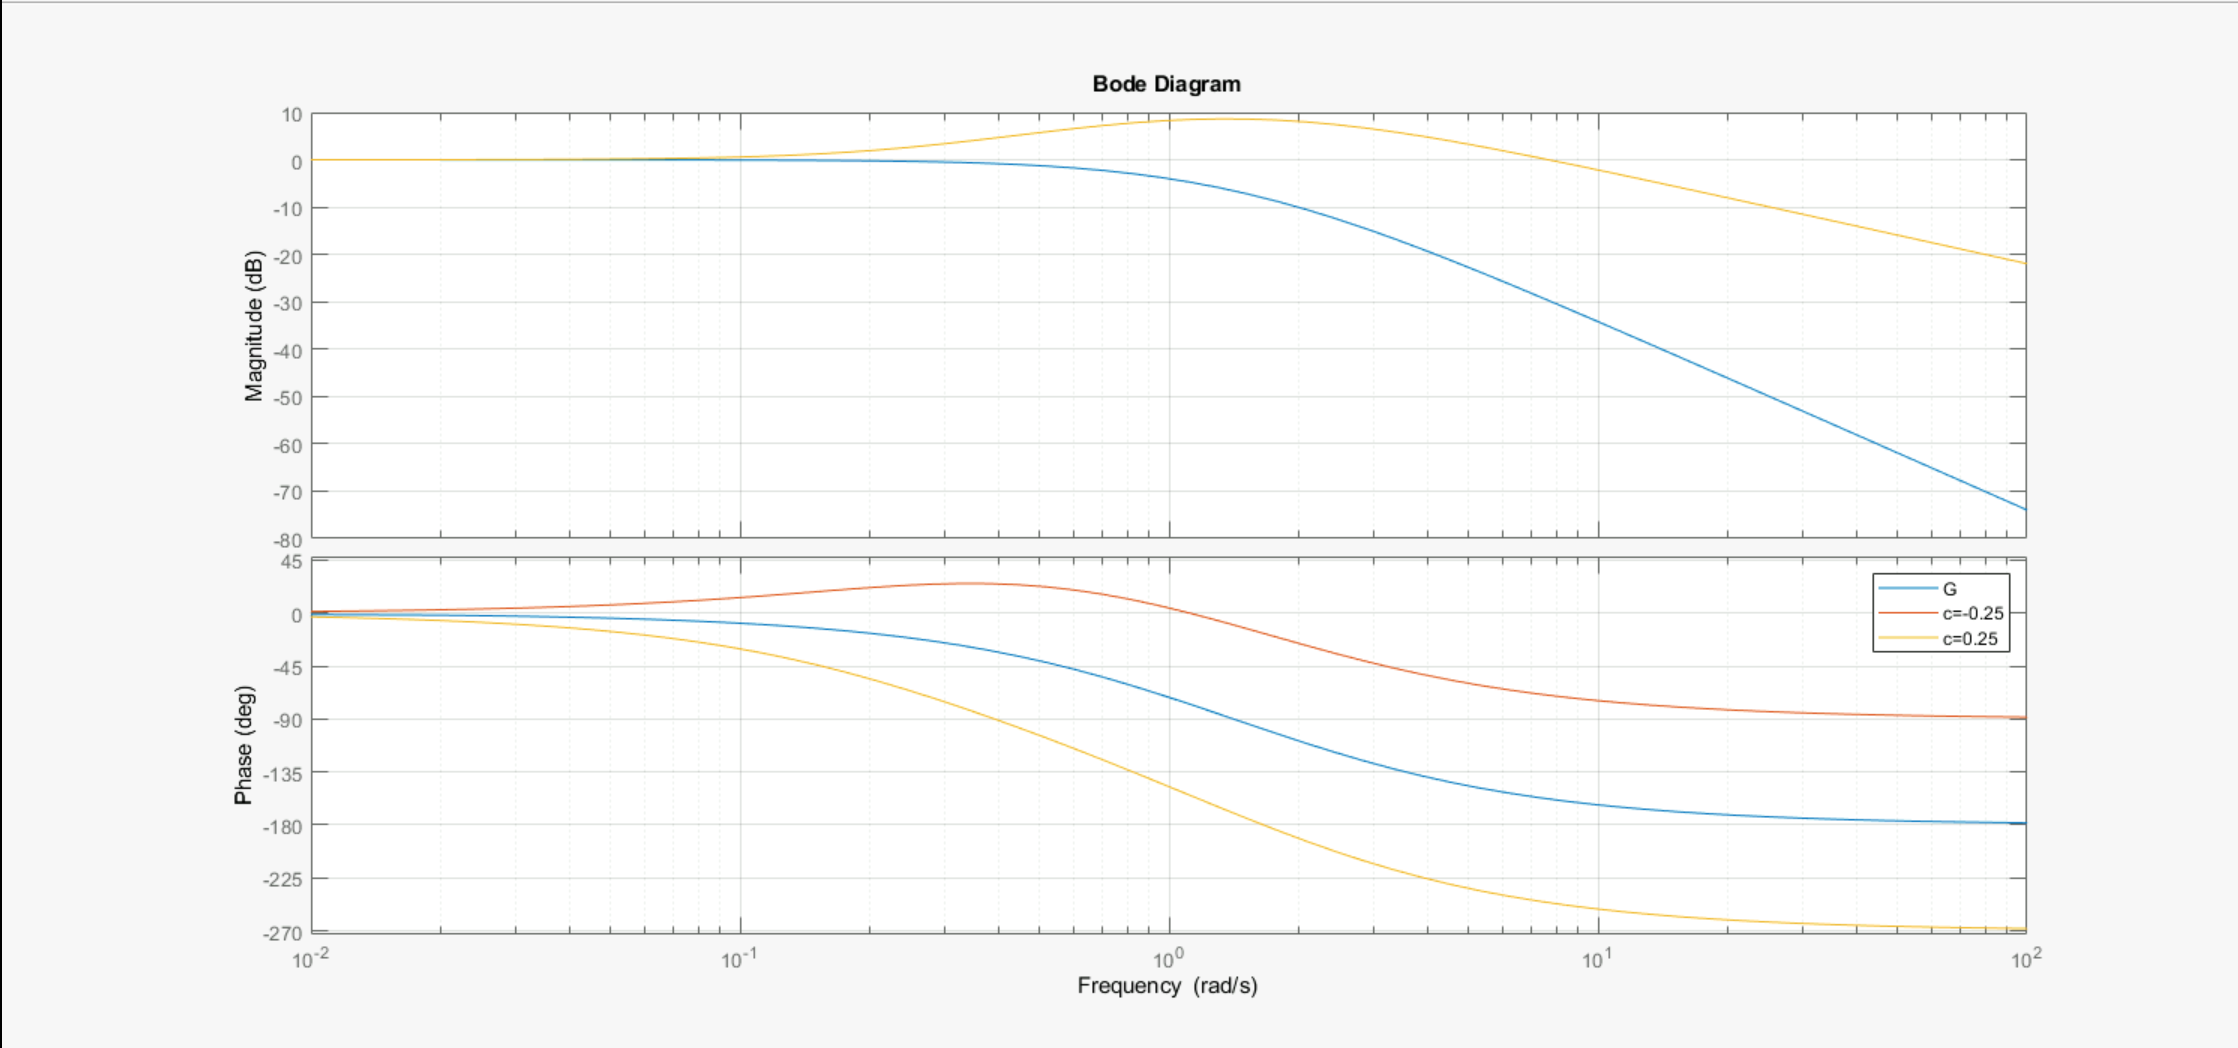
\includegraphics[width=0.75\textwidth]{figures/3_2/c=0.25.png}
\caption*{A2: $G$, $G_{c=-0.25}$, $G_{c=0.25}$ ($\alpha=0.25$).}
\end{figure}
\begin{figure}[H]
\centering
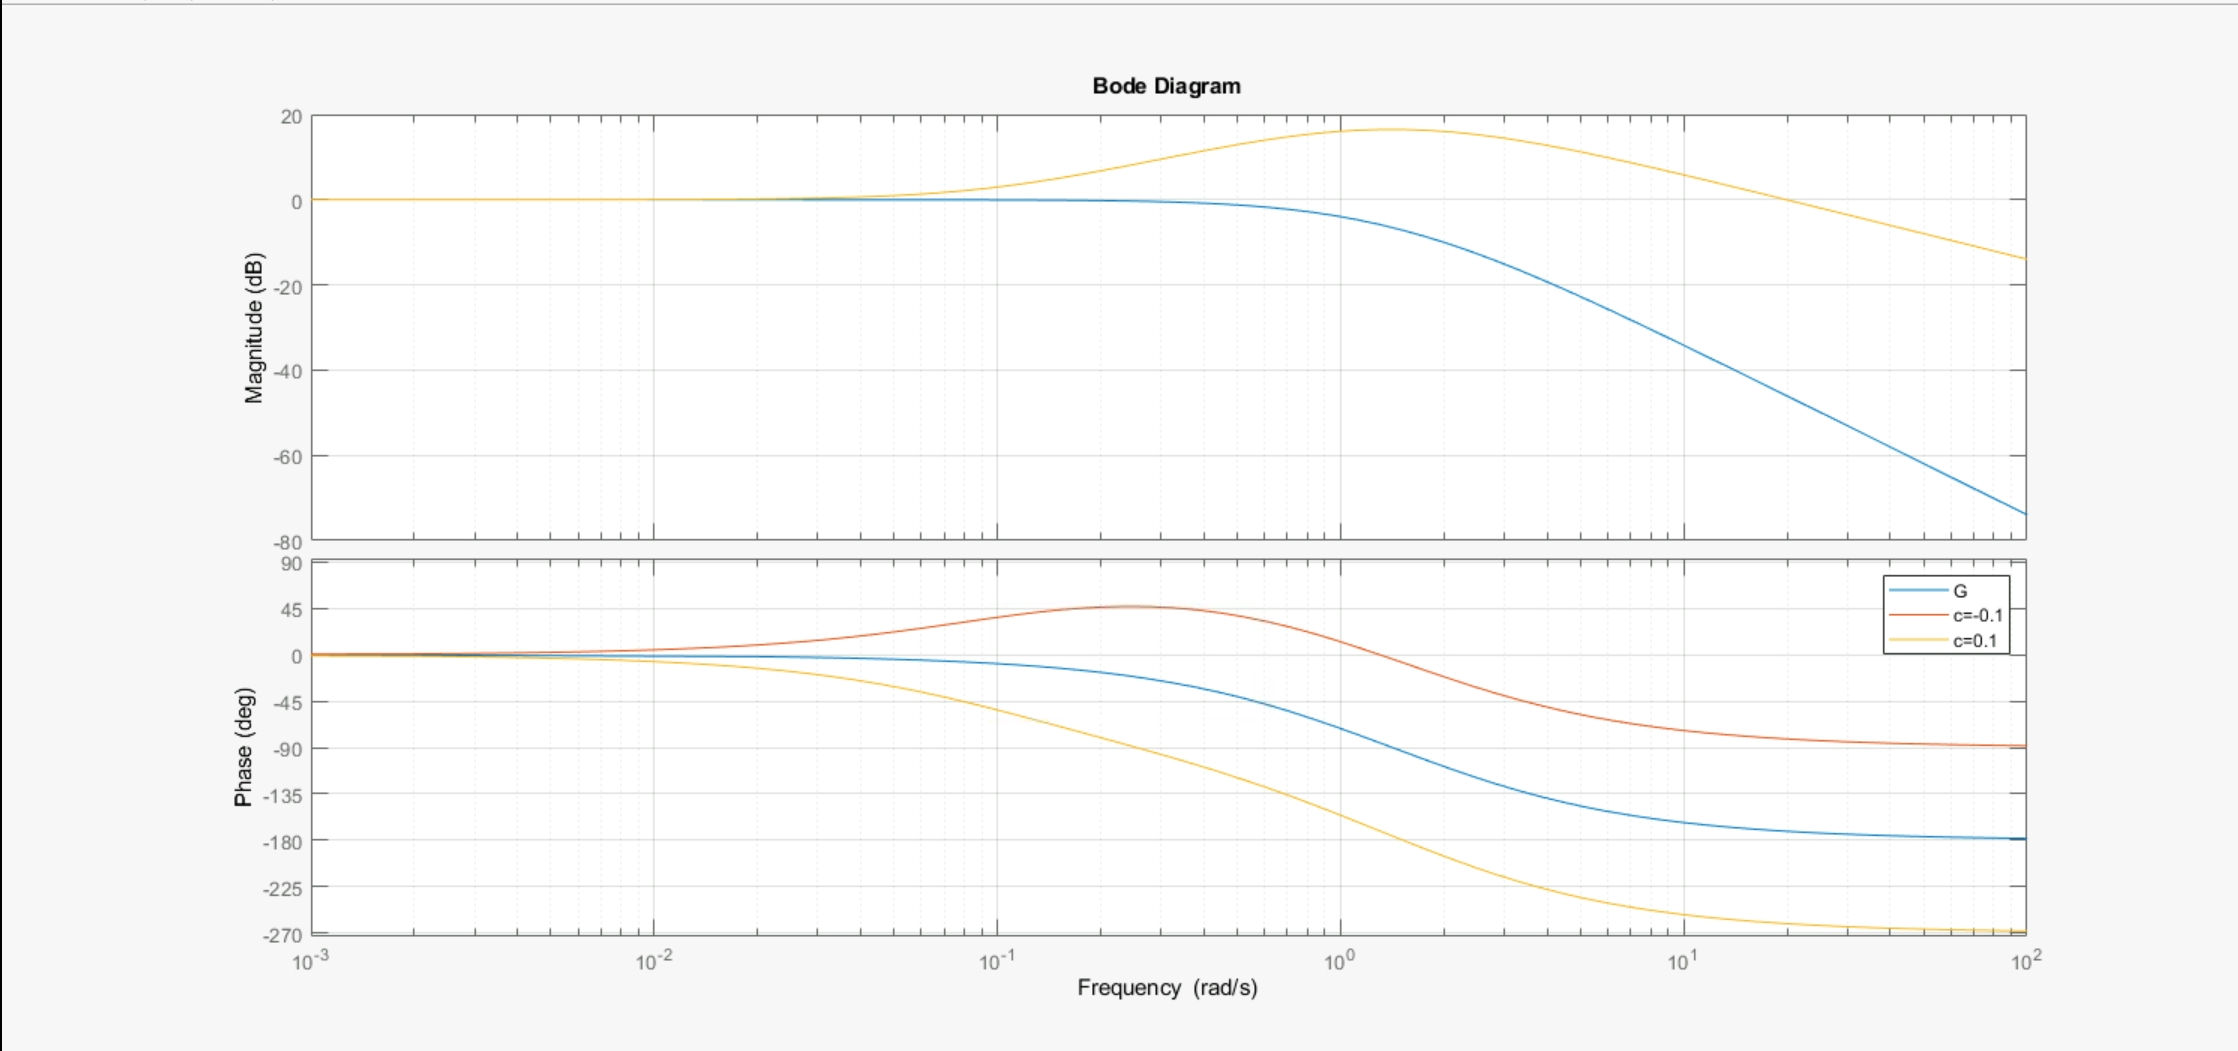
\includegraphics[width=0.75\textwidth]{figures/3_2/c=0.1.png}
\caption*{A3: $G$, $G_{c=-0.1}$, $G_{c=0.1}$ ($\alpha=0.1$).}
\end{figure}